Besides the dominant backgrounds discussed above, other SM backgrounds with
small cross sections were also considered and estimated for this analysis.
These include the diboson ($WW$, $WZ$, $ZZ$) processes, multiboson ($WWW$,
$WWZ$, $WZZ$, $ZZZ$) processes, the associated production with a top quark
pair ({\ensuremath{{\ttbar{}\mathrm{H}}}\xspace}, {\ensuremath{{\ttbar{}\mathrm{G}}}\xspace}, \ttbarW, and
\ttbarZ), and others ($tWZ$, $WZG$, $WWG$). 
Due to the requirement that at least one reconstructed top quark candidate be present, the backgrounds associated
with top quarks are expected to have higher selection efficiency than those without top quarks.  The
Feynman diagrams for the dominant \ttbarW and \ttbarZ production mechanisms in
proton-proton collisions are shown in Fig~\ref{fig:ttV_feynman}. 

\begin{figure}[htb]
  \centering
  $\vcenter{\hbox{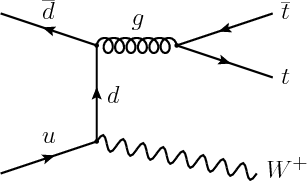
\includegraphics[width=0.35\textwidth]{sections/mc4/Backgrounds/TTZRare/figures/TTW}}}$
  \hspace{0.4 in}
  $\vcenter{\hbox{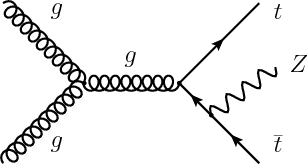
\includegraphics[width=0.37\textwidth]{sections/mc4/Backgrounds/TTZRare/figures/TTZ}}}$
  \caption{Dominant leading order Feynman diagrams for $\ttbarW^{+}$ and
  $\ttbarZ$ production at the LHC. The charge conjugate process of
  $\ttbarW^{+}$ produces $\ttbarW^{-}$.}
  \label{fig:ttV_feynman}
\end{figure}

The lost lepton and hadronic $\tau$ background use a data driven method, which therefore automatically takes into account the leptonically decaying $W$ and $Z$ components of these
backgrounds. The invisible $Z$ background method uses simulation only to derive scale factors. So only the hadronically decaying $W$ and $Z$,
$Z\rightarrow\nu\nu$ components of these rare backgrounds need to be explicitly addressed. To remove the
overlap between the prediction and the lost lepton and hadronic tau background
prediction, a veto on the generator level leptonically decaying $W$ and $Z$ is
applied.

\subsubsection{\texorpdfstring{\ttbarZ Background}{\ttbarZ Background}}
\label{sss:ttZ}

Similarly to the $Z\rightarrow\nu\nu$+jets background, \ttbarZ is an
irreducible background when the $Z$ decays to $\nu \nu$ and both top quarks decay
hadronically.  The \ttbarZ cross section at 13~TeV is 782.6 pb. The predicted
yield of \ttbarZ events in the search bins is less than 10\% of the total
background. Given the small cross section associated with this process, we
rely on simulation to generate a prediction, although this estimation is
validated using data. A validation study is performed in the
three-lepton channel following the \ttbarZ normalization exercise within the
SUSY group. The three-lepton channel is defined by the following selection:

\begin{itemize}
  \item Satisfies all filters that remove detector- and beam-related noise: 
    \begin{itemize}
      \item HBHE noise filter, 
      \item HBHEiso noise filter, 
      \item ECAL dead cell trigger primitive filter,
      \item Primary vertex filter,
      \item Bad EE super crystal filter,
      \item Global tight beam halo filter,
      \item Bad muon filter,
      \item Bad charged hadron filter,
      \item Loose JetID event filter.
    \end{itemize}
  \item Satisfies the trigger, here we only consider the single muon trigger
    \begin{itemize}
      \item \texttt{HLT\_Mu50\_v*}.
      \item \texttt{HLT\_IsoMu24\_v*}.
      \item \texttt{HLT\_IsoTKMu24\_v*}.
    \end{itemize}
  \item Has exactly 3 leptons
    \begin{itemize}
			\item Highest $p_{T}$ lepton, which is required by the trigger to be a muon, with $p_{T}>$ 40 GeV
			\item Leptons with the second and third largest $p_{T}$ with $p_{T}>$ 20 GeV
    \end{itemize}
  \item Has one reconstructed $Z$ boson within the mass window between 81 and 101 GeV
	\item At least 4 jets with $p_{T}>$ 40 GeV
	\item At least 2 b-tagged jets with $p_{T}>$ 30 GeV
  \item \MET $>$ 30 GeV
\end{itemize}

The list of MC samples for \ttbarZ and other rare backgrounds is given in
Table~\ref{tab:ttzNorm}. The \ttbarZ and other rare backgrounds are normalized to the SM
prediction. The measured yield of \ttbarZ and other rare backgrounds are compared with
single-muon data as shown in Fig~\ref{fig:ttZSUSY}, as a function of the
reconstructed $Z$ boson mass. The observed \ttbarZ rate is calculated by
subtracting the backgrounds yields from the data yield. The derived \ttbarZ scale
factor is $1.03 \pm 0.31$. The predicted \ttbarZ rate is consistent with data within the
statistical uncertainty. Thus we don't apply a scale factor for the \ttbarZ
yield in this analysis. A 30\% systematic uncertainty is assigned to the
\ttbarZ background prediction.

\begin{table}[hp]
  \centering
  \caption{The list of MC samples for \ttbarZ and other rare backgrounds}
  \label{tab:ttzNorm}
  \footnotesize
  \begin{tabular}{ll}
    \hline \hline
    Process & Dataset names \\
    \hline
    \ttbarZ & TTZToLLNuNu\_M-10\_TuneCUETP8M1\_13TeV-amcatnlo-pythia8 \\
    \hline
    \multirow{15}{*}{Rare} 
    & ttHToNonbb\_M125\_13TeV\_powheg\_pythia8   \\
    & VHToNonbb\_M125\_13TeV\_amcatnloFXFX\_madspin\_pythia8\\
    & GluGluHToZZTo4L\_M125\_13TeV\_powheg2\_JHUgenV6\_pythia8\\
    & ST\_tWll\_5f\_LO\_13TeV-MadGraph-pythia8\\
    & tZq\_ll\_4f\_13TeV-amcatnlo-pythia8\_TuneCUETP8M1\\
    & TTWJetsToLNu\_TuneCUETP8M1\_13TeV-amcatnloFXFX-madspin-pythia8\\
    & WZTo3LNu\_TuneCUETP8M1\_13TeV-amcatnloFXFX-pythia8\\
    & ZZTo4L\_13TeV\_powheg\_pythia8\\
    & WWZ\_TuneCUETP8M1\_13TeV-amcatnlo-pythia8\\
    & WZZ\_TuneCUETP8M1\_13TeV-amcatnlo-pythia8\\
    & ZZZ\_TuneCUETP8M1\_13TeV-amcatnlo-pythia8\\
    & WZG\_TuneCUETP8M1\_13TeV-amcatnlo-pythia8 \\
    & WWG\_TuneCUETP8M1\_13TeV-amcatnlo-pythia8 \\
    & WWW\_4F\_TuneCUETP8M1\_13TeV-amcatnlo-pythia8\\
    & TTTT\_TuneCUETP8M1\_13TeV-amcatnlo-pythia8\\
    \hline
    \multirow{2}{*}{NonPrompt} & 
    TTJets\_DiLept\_TuneCUETP8M1\_13TeV-madgraphMLM-pythia8\\
   & DYJetsToLL\_M-50\_HT-*\_TuneCUETP8M1\_13TeV-madgraphMLM-pythia8\\
    \hline
    \hline 
  \end{tabular}
\end{table}


\begin{figure}[htbp]
  \begin{center}
    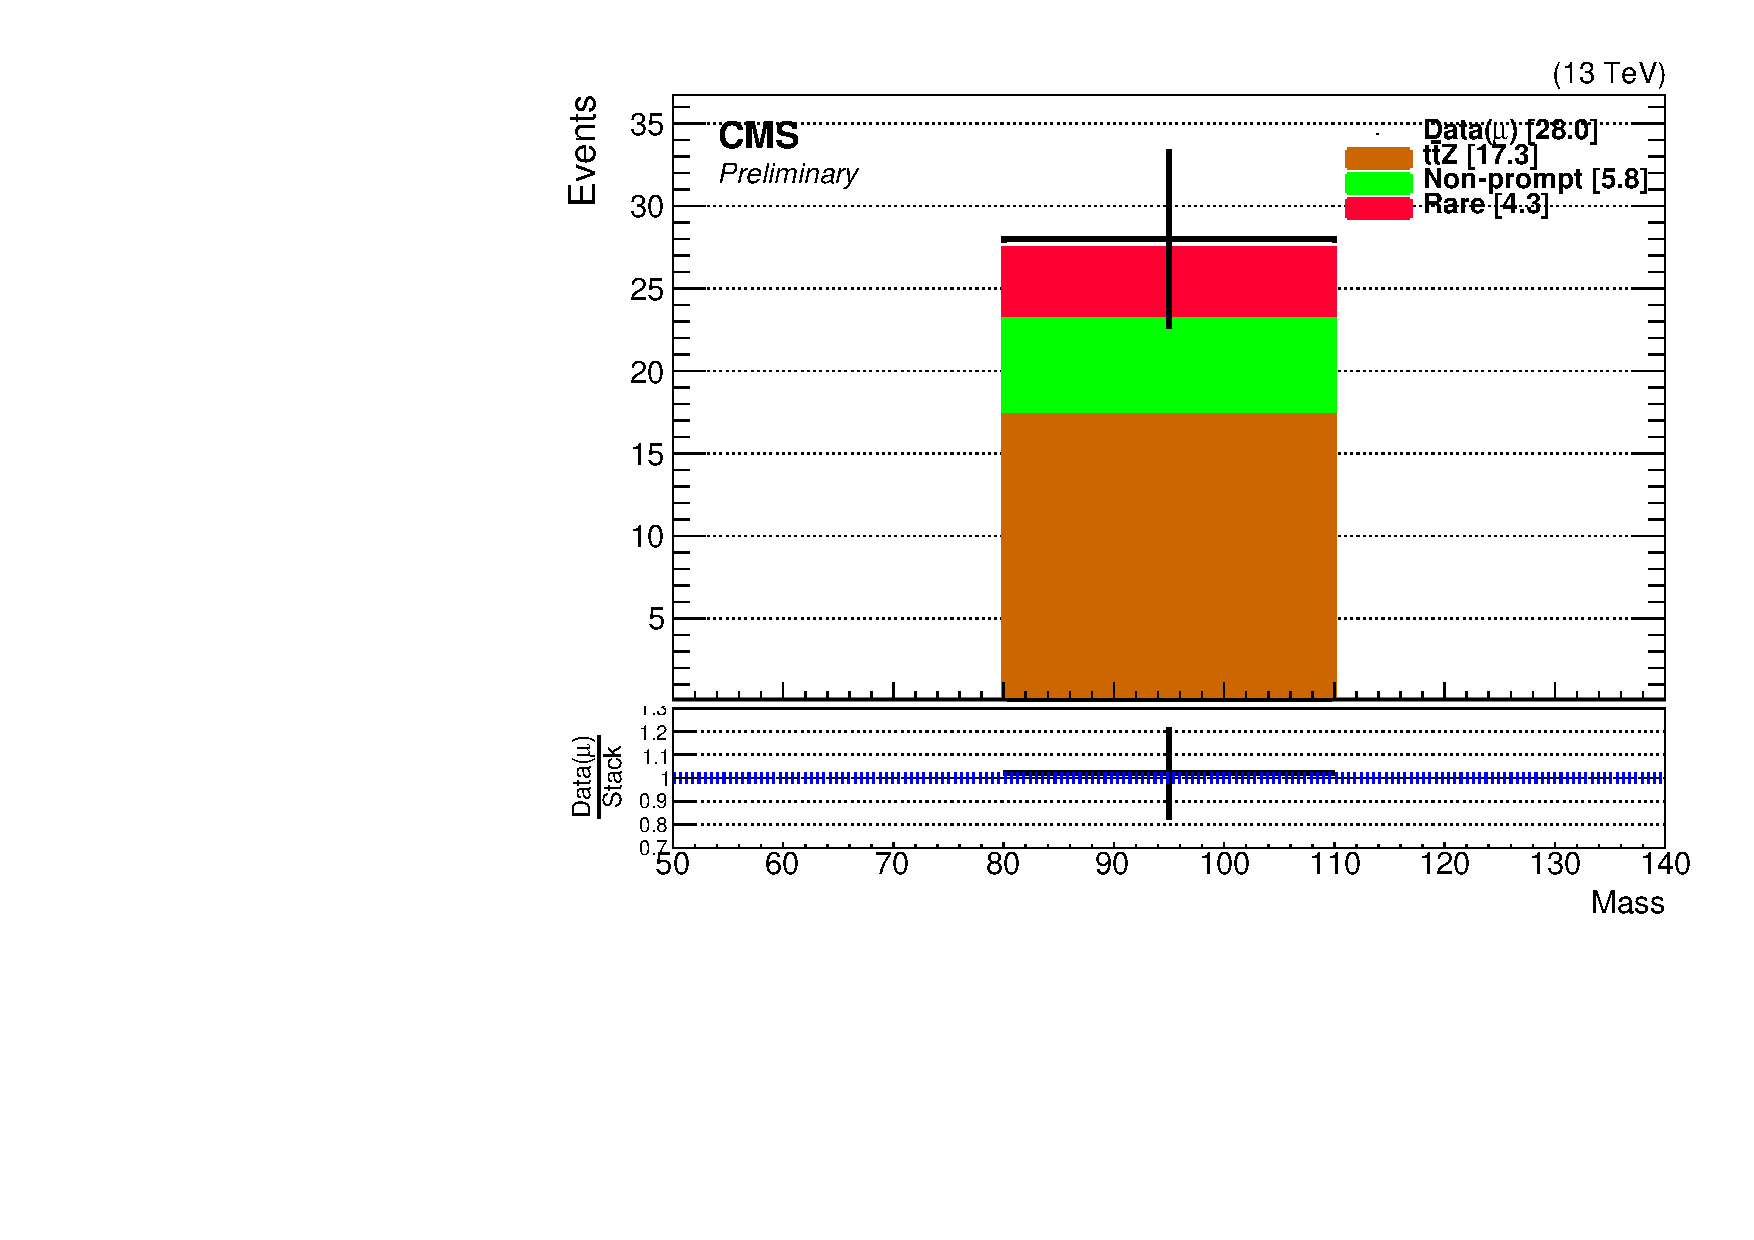
\includegraphics[width=0.79\textwidth]{sections/mc4/Backgrounds/TTZRare/figures/RecoZMass_7.pdf}
  \end{center}
  \caption{\ttbarZ validation in the three-leptons channels from the
  Single Muon data. The error bar denotes the statistical uncertainty.}
  \label{fig:ttZSUSY}
\end{figure}


Systematic uncertainties come from the choice of the renormalization/factorization
scale and PDF in the \ttbarZ MC samples are shown in
Fig~\ref{fig:ttZSysUncern}.  Other systematic uncertainties including ISR
reweighing, pileup correction, $b$--tagging scale factor are also considered.


\begin{figure}[htbp]
  \begin{center}
    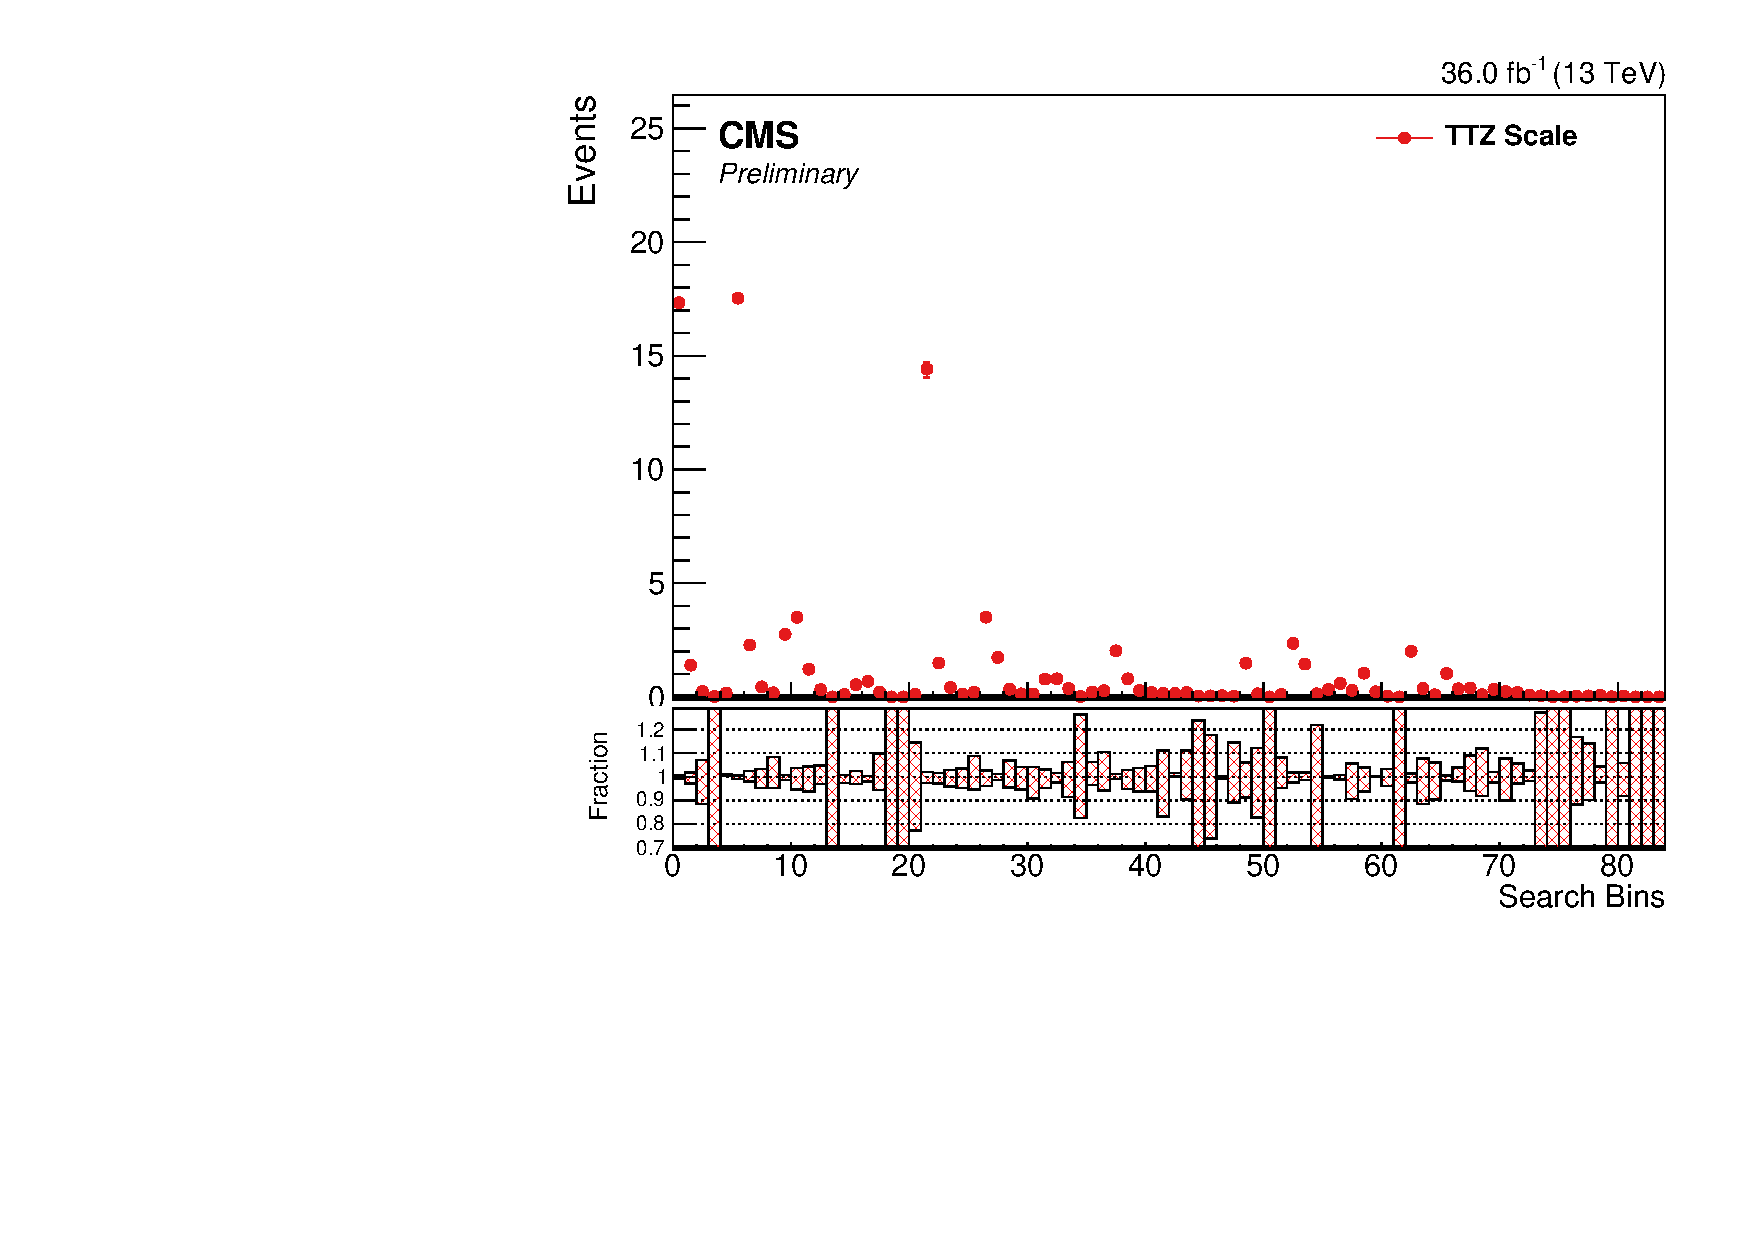
\includegraphics[width=0.49\textwidth]{sections/mc4/Backgrounds/TTZRare/figures/TTZ_Scale.pdf}
    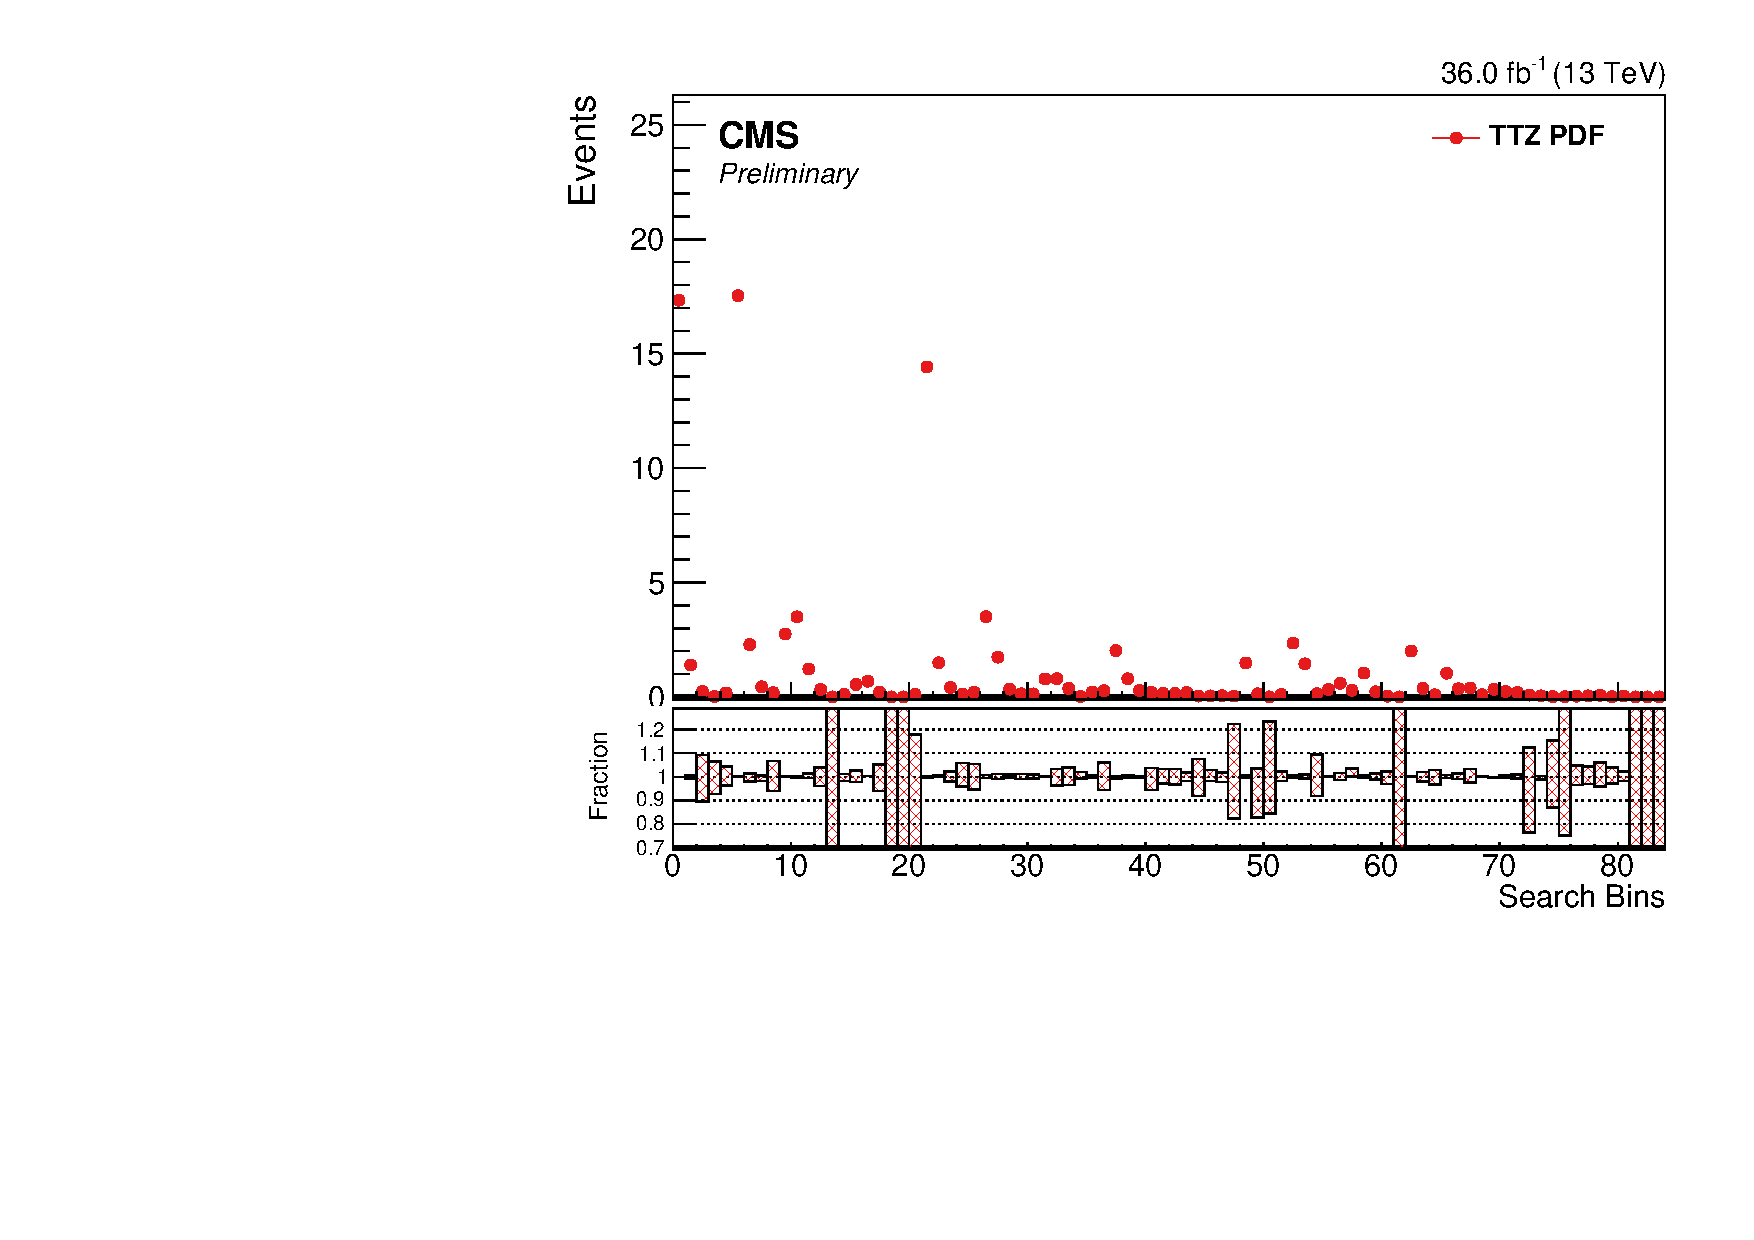
\includegraphics[width=0.49\textwidth]{sections/mc4/Backgrounds/TTZRare/figures/TTZ_PDF.pdf}
  \end{center}
  \caption{Systematic uncertainties from different sources that contribute to 
  the \ttbarZ background prediction, normalized to $36$~fb$^{-1}$.}
  \label{fig:ttZSysUncern}
\end{figure}

\subsubsection{Yields of Other SM Backgrounds}
\label{sss:otherSM}
The yields of the \ttbarZ and other rare backgrounds are derived from MC samples, normalized to the
SM predicted cross section. A generator-level veto of the leptonically decaying
$W$ and $Z$ bosons is applied to avoid double-counting with the lost-lepton and
hadronic tau backgrounds. Except for \ttbarZ process, the other backgrounds are
combined as the rare background. Their yield with statistical uncertainties is
shown in Fig~\ref{fig:ttZRareYeild}. Additional systematic uncertainties come from the choice
of renormalization/factorization scale and PDF in the rare MC samples, ISR
reweighting, pileup correction, and b-tagging scale factors.

\begin{figure}[htbp]
  \begin{center}
    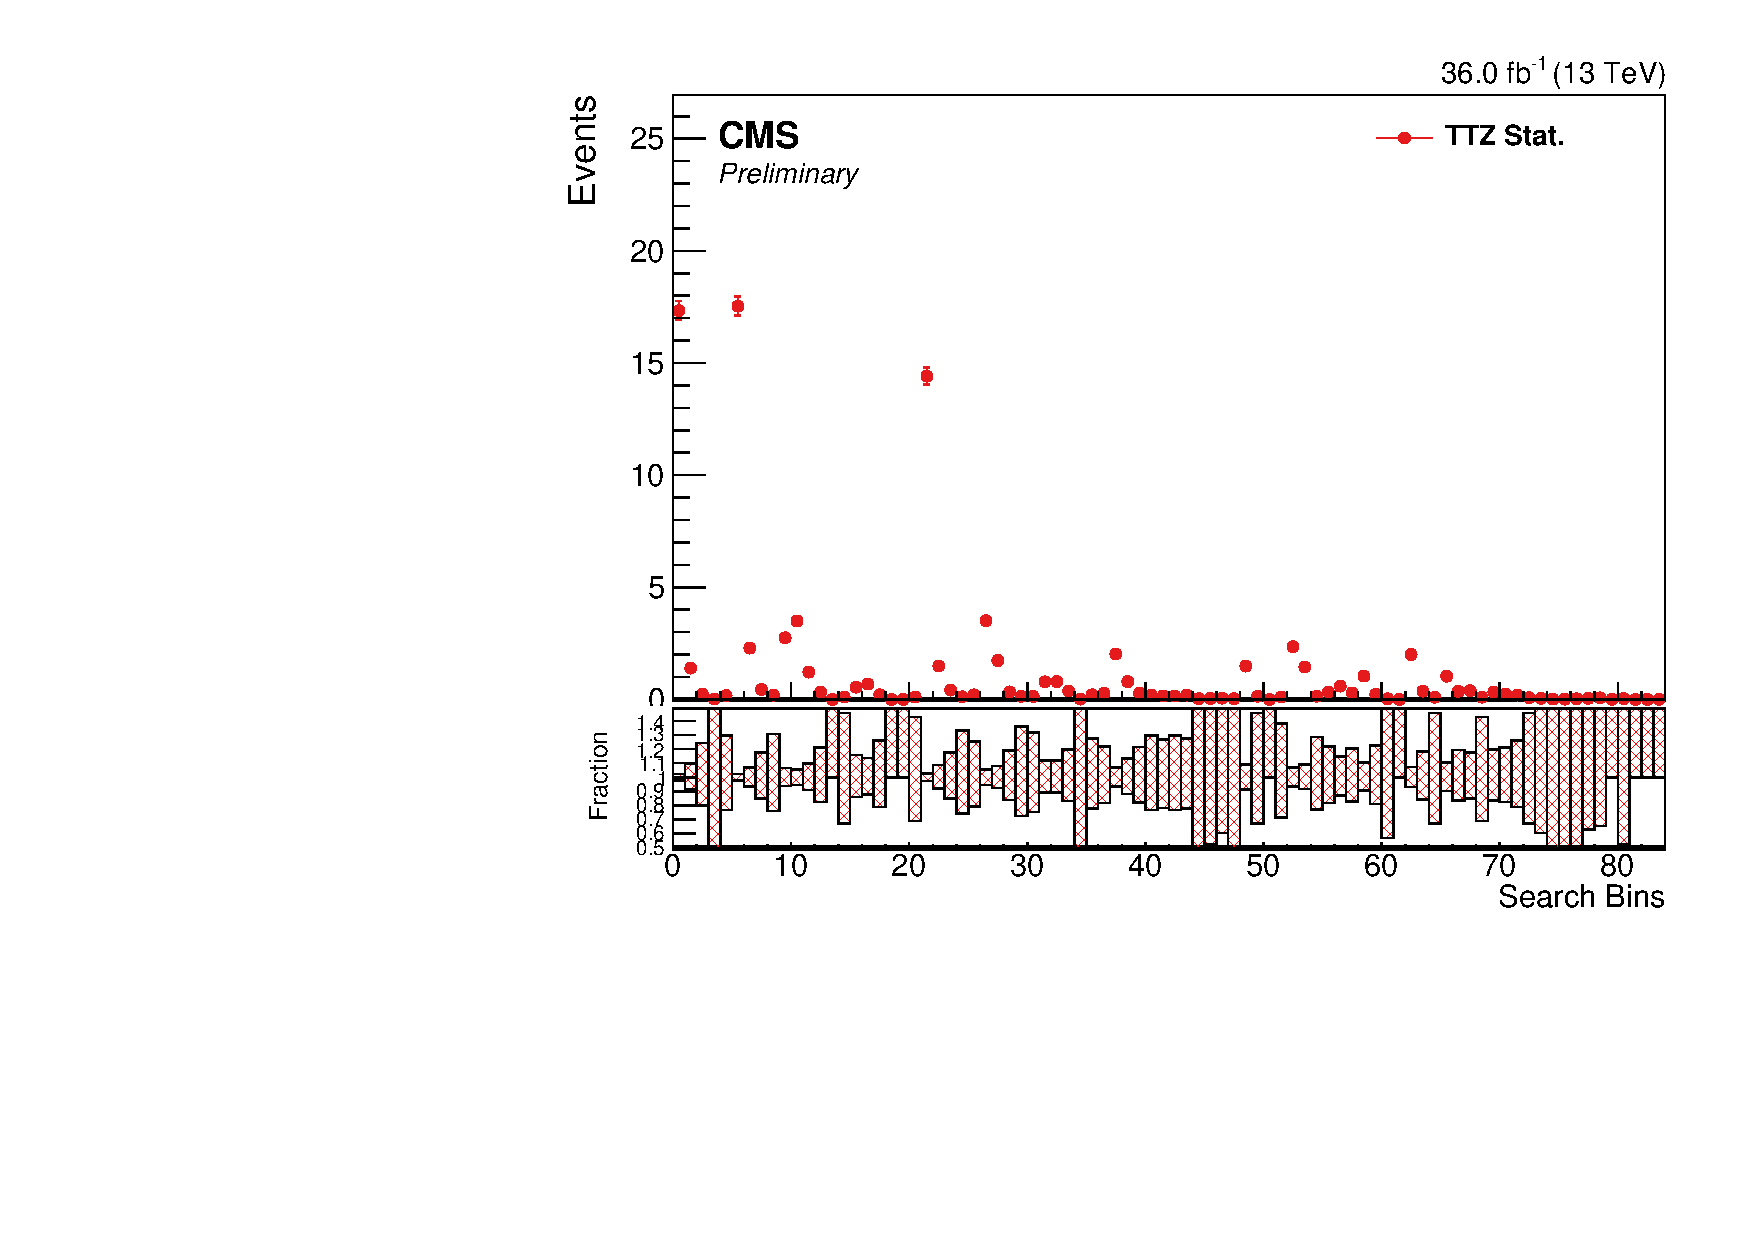
\includegraphics[width=0.49\textwidth]{sections/mc4/Backgrounds/TTZRare/figures/TTZ_Stat.pdf}
    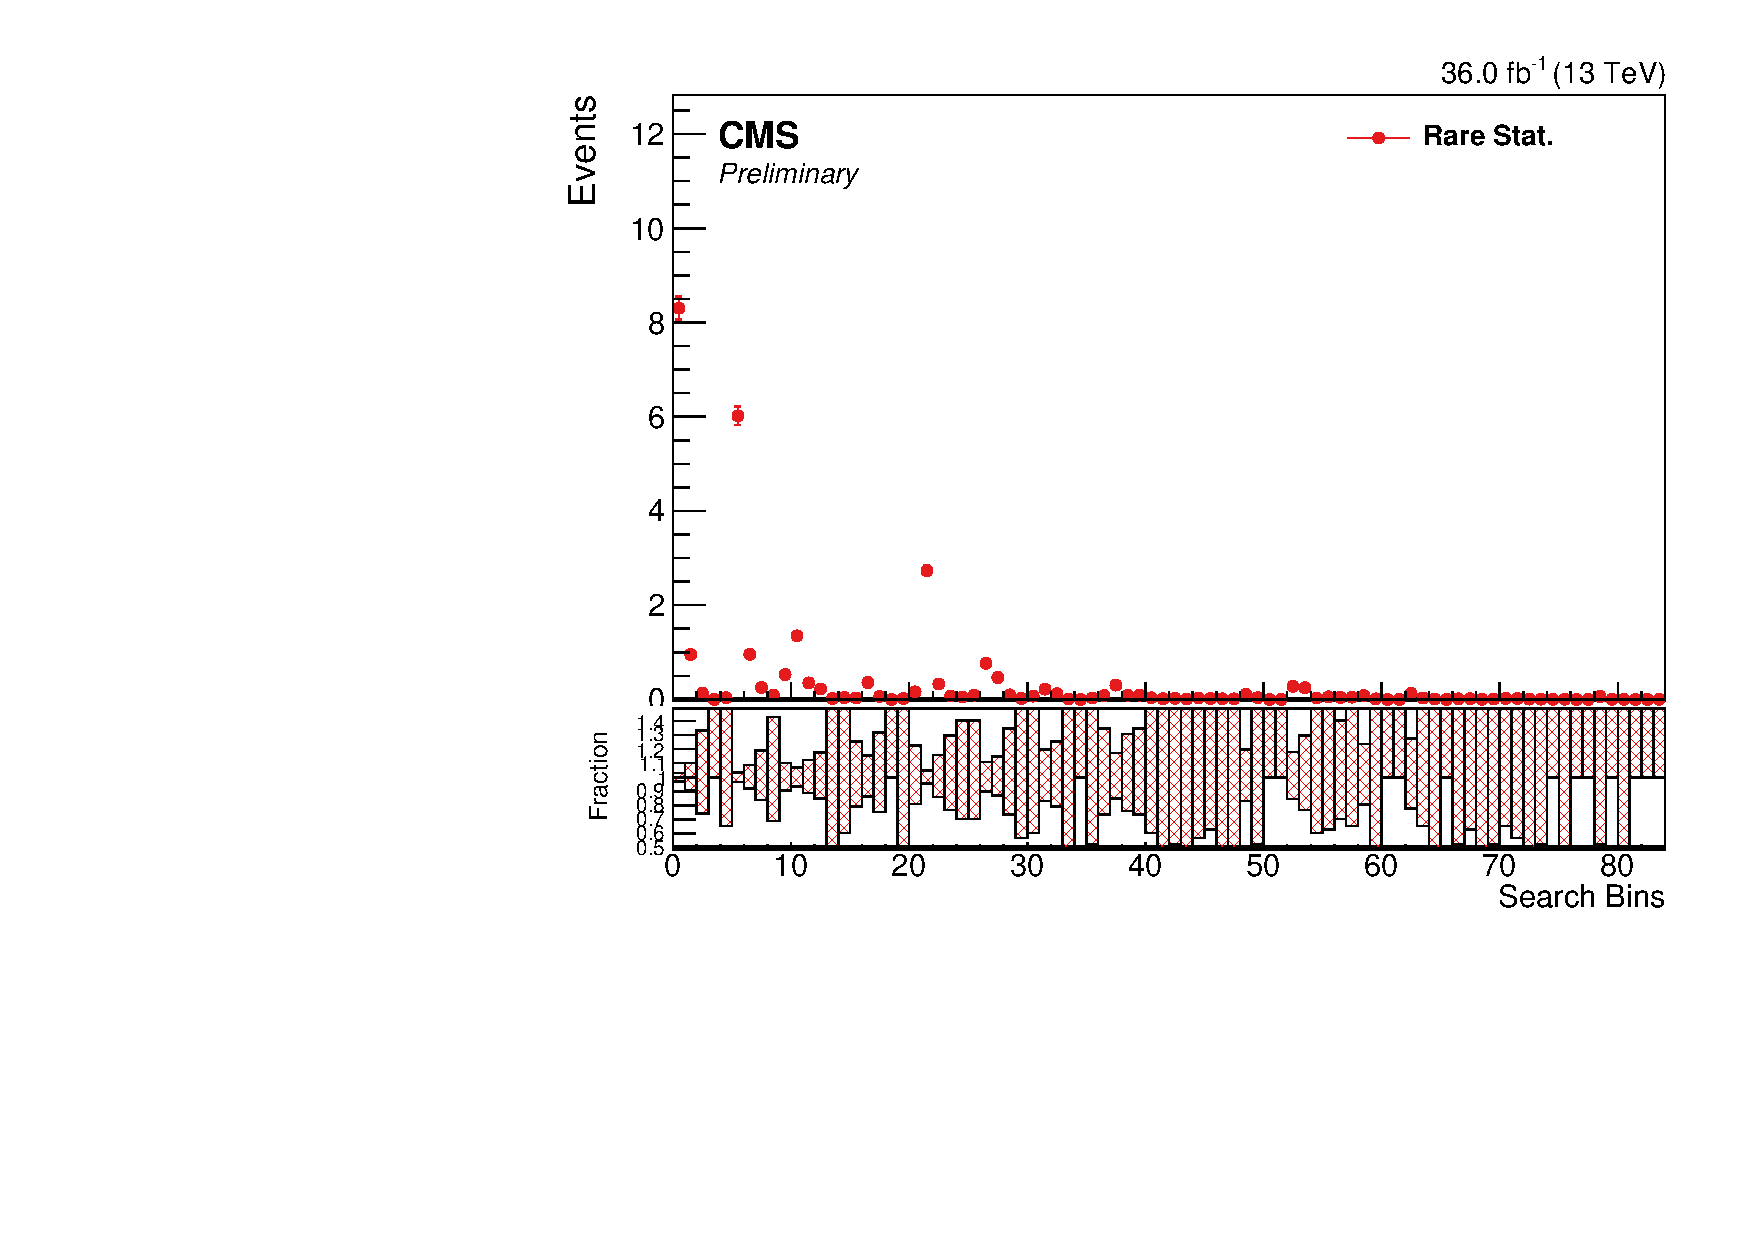
\includegraphics[width=0.49\textwidth]{sections/mc4/Backgrounds/TTZRare/figures/Rare_Stat.pdf}
  \end{center}
  \caption{Yield of the \ttbarZ and rare background prediction normalized to
  $36$~fb$^{-1}$.}
  \label{fig:ttZRareYeild}
\end{figure}
